% ============================================================================
%  COMPILE WITH XeLaTeX  (twice, so the point total resolves)
%  Overleaf: Menu -> Compiler -> XeLaTeX
%  Requires: bnhandout.sty and fonts/Kalpurush.ttf in the project
% ============================================================================
\documentclass[11pt]{article}
\usepackage{bnhandout}          % add [nosol] for a student edition

\hauthor[https://sites.google.com/view/jugantordey/home]{Jugantor Dey}
\hseries{Mathematics for the Physics Olympiad}

\begin{document}

\handouttitle{Chapter 16 : Differentials \& Differential Elements}

\noindent
এই অধ্যায়ের একমাত্র পূর্বশর্ত ১৫ নম্বর অধ্যায়: derivative-এর সংজ্ঞা,
chain rule, $\ln x$-এর derivative, এবং আংশিক derivative নিয়ে যা বলা হয়েছিল
সেটুকু। ১১ নম্বর অধ্যায়ের solid angle আর ১২ নম্বর অধ্যায়ের
cylindrical ও spherical স্থানাঙ্কও তৃতীয় অনুচ্ছেদে সরাসরি লাগবে।

১৫ নম্বর অধ্যায়ে বলা হয়েছিল যে $\dfrac{dy}{dx}$ একটি অখণ্ড প্রতীক,
ভগ্নাংশ নয়, আর $dy$ ও $dx$ আলাদা করে কী বোঝায় তা পরে আসবে। সেটাই এই
অধ্যায়।

কেন এটি আলাদা অধ্যায় পাওয়ার যোগ্য, সেটা বলে রাখি। পদার্থবিজ্ঞানের বইয়ে
প্রতিটি ইন্টিগ্রাল শুরু হয় একটি বাক্য দিয়ে: ``ছোট একটি টুকরো নাও, তার অবদান
$dm$ বা $dV$ বা $dW$ লেখো''। যে শিক্ষার্থী কেবল $\dfrac{dy}{dx}$ চেনে, সে ওই
বাক্যটি পড়ে থমকে যায়, কারণ সেখানে $d$ চিহ্নটি সম্পূর্ণ অন্য কাজ করছে। ফলে
ইন্টিগ্রাল শেখা হয় সূত্র হিসেবে, আর সেটআপ করা শেখা হয় না। অথচ অলিম্পিয়াডে
কঠিন কাজটা প্রায় সবসময় সেটআপেই, হিসাবে নয়; হিসাবটা অনেক সময় দেওয়াই থাকে, হিসাব পর্যন্ত ঠিকভাবে পৌঁছানোই চ্যালেঞ্জ।

এখানে ইন্টিগ্রাল সল্ভ করা শেখানো হবে না; সেটি ১৭ নম্বর অধ্যায়ের কাজ। এখানে শেখানো হবে ইন্টিগ্রালের ইন্টিগ্র্যান্ড সেটাপ করা। এই অধ্যায়ে মোট
\totalpoints\ পয়েন্ট আছে।  

\section{ডেরিভেটিভ বনাম ডিফারেনশিয়াল}

$f'(a)$ সংখ্যাটি একটি limit, এবং সেটি এক টুকরো। কিন্তু Leibniz-এর লেখা
$\dfrac{dy}{dx}$ দেখতে ভগ্নাংশের মতো, আর সেটা কাকতালীয় নয়। একটু কাজ করলে
লব ও হরকে আলাদা অর্থ দেওয়া যায়, এমনভাবে যে ভাগফলটি সত্যিই $f'(x)$ হয়।

\begin{idea}[Differential]
$y = f(x)$ ধরো, যেখানে $f$ differentiable। এখন $dx$-কে একটি স্বাধীন চলক ধরো,
অর্থাৎ যেকোনো বাস্তব সংখ্যা। তারপর $dy$-কে সংজ্ঞায়িত করো
\[
  dy = f'(x)\,dx .
\]
$dy$-কে বলে $y$-এর differential। এখানে $dy$ নির্ভর করে দুটি জিনিসের উপর:
কোন বিন্দুতে আছি ($x$) এবং কতটুকু নড়ছি ($dx$)।
\end{idea}

খেয়াল করো যুক্তির ক্রমটা। derivative আগে সংজ্ঞায়িত হয়েছে (limit দিয়ে);
তারপর $dy$-কে এমনভাবে সংজ্ঞায়িত করা হলো যাতে $dx \neq 0$ হলে
\[
  \frac{dy}{dx} = f'(x)
\]
সত্যি সত্যিই একটি ভাগফল হয়। উল্টো দিকে যাওয়া হয়নি; ``$dy$ ও $dx$ দুটি ছোট
সংখ্যা, তাদের ভাগ করলে derivative পাওয়া যায়'' এই গল্পটা সংজ্ঞা নয়।

জ্যামিতিক অর্থটা ছবিতে সবচেয়ে পরিষ্কার।

\begin{center}
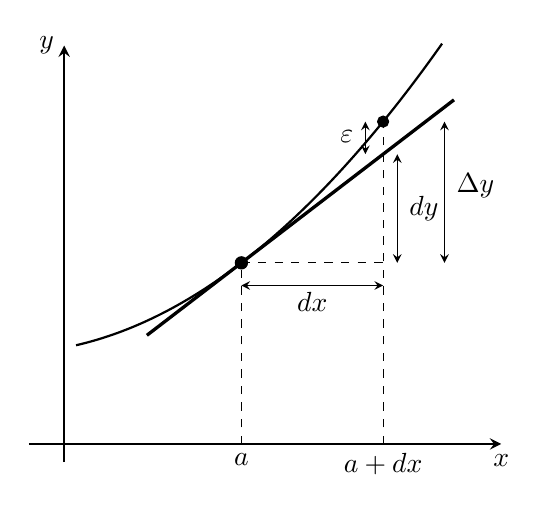
\begin{tikzpicture}[x=1.5cm,y=1.15cm,>=stealth]
  \draw[thick,->] (0.2,0) -- (4.2,0) node[below] {$x$};
  \draw[thick,->] (0.5,-0.2) -- (0.5,4.4) node[left] {$y$};
  \draw[thick,domain=0.6:3.7,samples=80,variable=\x] plot ({\x},{0.25*\x*\x+1});
  \draw[very thick] (1.2,1.2) -- (3.8,3.8);
  \draw[fill] (2,2) circle (2.2pt);
  \draw[dashed] (2,0) -- (2,2);
  \draw[dashed] (2,2) -- (3.2,2);
  \draw[dashed] (3.2,0) -- (3.2,3.56);
  \draw[fill] (3.2,3.56) circle (2pt);
  \node[below] at (2,0) {$a$};
  \node[below] at (3.2,0) {$a+dx$};
  \draw[<->] (2,1.75) -- (3.2,1.75);
  \node[below] at (2.6,1.78) {$dx$};
  \draw[<->] (3.32,2) -- (3.32,3.2);
  \node[right] at (3.34,2.6) {$dy$};
  \draw[<->] (3.72,2) -- (3.72,3.56);
  \node[right] at (3.74,2.85) {$\Delta y$};
  \draw[<->] (3.05,3.2) -- (3.05,3.56);
  \node[left] at (3.03,3.4) {$\varepsilon$};
\end{tikzpicture}
\end{center}

$a$ থেকে $a+dx$-এ গেলে ফাংশনের প্রকৃত পরিবর্তন
\[
  \Delta y = f(a+dx) - f(a) ,
\]
 যা বক্ররেখার দুইটি নিকটবর্তী বিন্দুর উল্লম্ব দূরত্ব অর্থাৎ ফাংশনের মানের পরিবর্তন। আর $dy = f'(a)\,dx$ হলো একই দূরত্ব সরলে (আনুভূমিকভাবে)
\emph{স্পর্শক} বরাবর যতটুকু ওঠা হতো (উল্লম্ব দিকে)। দুটি এক নয়; পার্থক্য
$\varepsilon = \Delta y - dy$।

এই $\varepsilon$-ই আসল কথা। ১৪ নম্বর অধ্যায়ে দেখা গিয়েছিল যে ছোট এলাকায়
বক্ররেখা প্রায় সরল; এখন সেটাই পরিমাপ করা যাচ্ছে। derivative-এর সংজ্ঞা বলছে
\[
  \frac{\Delta y}{dx} \;\longrightarrow\; f'(a) ,
\]
আর $dy/dx = f'(a)$ ধ্রুবক, তাই বিয়োগ করলে
\[
  \frac{\varepsilon}{dx} = \frac{\Delta y - dy}{dx}
  \;\longrightarrow\; 0 .
\]
অর্থাৎ $\varepsilon$ কেবল ছোট নয়, সে $dx$-এর তুলনায়ও ছোট। এই একটি বাক্যই
পরের সব কিছুর ভিত্তি।

\begin{example}
$y = x^{2}$ ধরো এবং $x = 3$ বিন্দুতে $dx = 0.1$ নাও। $dy$, $\Delta y$ ও
$\varepsilon$ নির্ণয় করো।
\end{example}

\begin{solbox}
$f'(x) = 2x$, তাই $f'(3) = 6$ এবং
\[
  dy = 6 \times 0.1 = 0.6 .
\]
প্রকৃত পরিবর্তন
\[
  \Delta y = (3.1)^{2} - 3^{2} = 9.61 - 9 = 0.61 .
\]
সুতরাং $\varepsilon = 0.01$।

কোথা থেকে এল সেটাও দেখা যায়: $(3+dx)^{2} - 9 = 6\,dx + (dx)^{2}$, অর্থাৎ
$\Delta y = dy + (dx)^{2}$ এবং $\varepsilon = (dx)^{2}$ হুবহু। $dx$ দশ গুণ
ছোট করলে $dy$ দশ গুণ ছোট হবে কিন্তু $\varepsilon$ একশ গুণ ছোট হবে; সেটাই
``$dx$-এর তুলনায় ছোট'' কথাটার মানে।
\end{solbox}

\prob{2} $y = x^{3}$ ধরো, $x = 2$ এবং $dx = 0.01$। $dy$, $\Delta y$ ও
$\varepsilon$ নির্ণয় করো এবং $\varepsilon$-এর আকার $dx$-এর সঙ্গে তুলনা করো।

\begin{sol}
$f'(x) = 3x^{2}$, তাই $f'(2) = 12$ এবং $dy = 12 \times 0.01 = 0.12$।

$\Delta y = (2.01)^{3} - 8 = 8.120601 - 8 = 0.120601$।

সুতরাং $\varepsilon = 0.000601$।

তুলনা: $\varepsilon / dx = 0.0601$, যা $dx = 0.01$-এর তুলনায় ছোট নয় বরং
বড় দেখাচ্ছে; কিন্তু ব্যাপারটা হলো $\varepsilon/dx \to 0$ যখন $dx \to 0$।
বীজগণিতে: $(2+dx)^{3} - 8 = 12\,dx + 6(dx)^{2} + (dx)^{3}$, তাই
$\varepsilon = 6(dx)^{2} + (dx)^{3}$ এবং $\varepsilon/dx = 6\,dx + (dx)^{2}
\to 0$। $dx$ দশ গুণ ছোট করলে $\varepsilon$ প্রায় একশ গুণ ছোট হবে।
\end{sol}

\prob{2} নিচের প্রতিটির জন্য $dy$ লেখো।
\begin{enumerate}
  \item $y = x\sin x$
  \item $y = e^{2x}$
  \item $y = \ln\left( 1+x^{2} \right)$
\end{enumerate}

\begin{sol}
প্রতিটিতে $dy = f'(x)\,dx$ বসাই।
\begin{enumerate}
  \item $dy = \left( \sin x + x\cos x \right)dx$।
  \item $dy = 2e^{2x}\,dx$।
  \item $dy = \dfrac{2x}{1+x^{2}}\,dx$।
\end{enumerate}
\end{sol}

\section{$dx$-এর অর্থ}

একই চিহ্ন $d$ তিন জায়গায় তিন রকম কাজ করে, আর সেটা না জানলে বিভ্রান্তি
অনিবার্য। তিনটি পাঠ আলাদা করে লিখে রাখি।

\begin{idea}[$d$-এর তিনটি পাঠ]
\begin{enumerate}
  \item $\dfrac{dy}{dx}$-এর ভেতরে: এটি একটি অখণ্ড প্রতীক, একটি limit-এর নাম।
        এখানে $dx$ আলাদা করে কিছু বোঝায় না।
  \item Differential হিসেবে: $dx$ একটি সাধারণ বাস্তব চলক এবং
        $dy = f'(x)\,dx$ একটি \emph{নির্ভুল} সমীকরণ, কোনো আসন্নীকরণ নয়।
        $dx$-কে ছোট হতেও হয় না।
  \item পদার্থবিজ্ঞানীর পাঠ: $dx$ মানে ``অসীম ছোট এক টুকরো $x$''। এটি কোনো
        বাস্তব সংখ্যা নয়, এবং এই অর্থে $dx$ কড়াভাবে সংজ্ঞায়িতও নয়।
\end{enumerate}
\end{idea}

তৃতীয় পাঠটি নিয়ে খোলাখুলি কথা বলা দরকার। ``অসীম ছোট সংখ্যা'' বলে বাস্তব
সংখ্যায় কিছু নেই: শূন্যের চেয়ে বড় অথচ সব ধনাত্মক সংখ্যার চেয়ে ছোট, এমন
বাস্তব সংখ্যা থাকতে পারে না। তবু পদার্থবিজ্ঞানে এই ভাষা কাজ করে, কারণ
$dx$-যুক্ত প্রতিটি বাক্য আসলে $\Delta x$ ও একটি limit নিয়ে লেখা একটি বাক্যের
সংক্ষিপ্ত রূপ। যেমন ``$dW = F\,dx$'' কথাটির পূর্ণ অর্থ: ছোট সরণ $\Delta x$-এ
কৃতকাজ প্রায় $F\,\Delta x$, আর মোট কাজ হলো এমন অসংখ্য টুকরোর যোগফলের limit।
এই limit নেওয়ার কাজটাই ১৭ নম্বর অধ্যায়ের integral।

সুতরাং তৃতীয় পাঠটি ভুল নয়, অসম্পূর্ণ। এখানে আমরা একে সুবিধাজনক সংক্ষেপ
হিসেবেই ব্যবহার করব, এবং মনে রাখব যে পেছনে একটি limit লুকিয়ে আছে।

\begin{idea}[Chain rule, differential আকারে]
$y = f(u)$ এবং $u = g(x)$ হলে
\[
  dy = f'(u)\,du, \qquad du = g'(x)\,dx
  \;\Longrightarrow\;
  dy = f'(u)\,g'(x)\,dx .
\]
অর্থাৎ differential-গুলো পরপর বসিয়ে দিলেই chain rule বেরিয়ে আসে।
\end{idea}

এই রূপটাই Leibniz-এর লেখার আসল সুবিধা। $\dfrac{dy}{dx} = \dfrac{dy}{du}
\cdot \dfrac{du}{dx}$ লিখলে মনে হয় $du$ কাটাকাটি গেল, আর সেটা এখানে
সত্যিই বৈধ, কারণ $du$ একটি সত্যিকারের সংজ্ঞায়িত রাশি। ১৭ নম্বর অধ্যায়ে
integral-এ চলক প্রতিস্থাপনের নিয়মটিও ঠিক এই একই কারণে কাজ করে।

\begin{remark}
কিন্তু এই কাটাকাটির অভ্যাসটা আংশিক derivative-এ নিয়ে যেয়ো না।
$\dfrac{\partial P}{\partial V}$-তে ``$\partial V$'' বলে আলাদা কোনো বস্তু নেই;
চিহ্নটির অর্থ নির্ভর করে কোন কোন চলক স্থির রাখা হয়েছে তার উপর, আর আলাদা
ভগ্নাংশে সেই তালিকা আলাদা। ১৫ নম্বর অধ্যায়ের আদর্শ গ্যাসের সমস্যাটি মনে
করো:
\[
  \frac{\partial P}{\partial V} \cdot \frac{\partial V}{\partial T} \cdot
  \frac{\partial T}{\partial P} = -1 ,
\]
কাটাকাটি করলে $+1$ আসত। এর চেয়ে পরিষ্কার প্রমাণ আর হয় না যে
$\partial$ ভগ্নাংশের লব বা হর নয়।
\end{remark}

\begin{example}
Differential ব্যবহার করে $y = \sin\left( x^{2} \right)$-এর $dy$ নির্ণয় করো।
\end{example}

\begin{solbox}
$u = x^{2}$ ধরি, তাই $y = \sin u$। তখন
\[
  du = 2x\,dx, \qquad dy = \cos u \; du .
\]
দ্বিতীয়টিতে প্রথমটি বসিয়ে
\[
  dy = \cos\left( x^{2} \right) \cdot 2x\,dx = 2x\cos\left( x^{2} \right)dx .
\]
১৫ নম্বর অধ্যায়ে chain rule দিয়ে ঠিক এই উত্তরই এসেছিল; পার্থক্য কেবল
লেখার ভঙ্গিতে। ভেতরের ফাংশনটিকে $u$ নাম দিয়ে ধাপে ধাপে এগোনো যায় বলে জটিল
ক্ষেত্রে এই ভঙ্গিটি কম ভুল করায়।
\end{solbox}

\prob{2} Differential আকারে chain rule ব্যবহার করে $y = \sqrt{1+3x}$-এর $dy$
নির্ণয় করো।

\begin{sol}
$u = 1+3x$ ধরি, তাই $y = u^{1/2}$ এবং
\[
  du = 3\,dx, \qquad dy = \tfrac{1}{2}u^{-1/2}\,du .
\]
বসিয়ে
\[
  dy = \frac{1}{2\sqrt{1+3x}} \cdot 3\,dx = \frac{3}{2\sqrt{1+3x}}\,dx .
\]
\end{sol}

\prob{3} chain rule-এ $\dfrac{dy}{du} \cdot \dfrac{du}{dx}$ লিখে $du$ কাটাকাটি
করা কেন বৈধ, অথচ আংশিক derivative-এ $\partial$ কাটাকাটি করা কেন অবৈধ, তা
ব্যাখ্যা করো। ১৫ নম্বর অধ্যায়ের আদর্শ গ্যাসের ফলটি উদাহরণ হিসেবে ব্যবহার
করো।

\begin{sol}
বৈধ হওয়ার কারণ: এই অনুচ্ছেদে $du$ ও $dx$ দুটিকেই আলাদা রাশি হিসেবে
সংজ্ঞায়িত করা হয়েছে, আর $dy = f'(u)\,du$ এবং $du = g'(x)\,dx$ দুটি
নির্ভুল সমীকরণ। তাই $\dfrac{dy}{du}$ ও $\dfrac{du}{dx}$ সত্যিকারের ভগ্নাংশ
এবং তাদের গুণফলে $du$ কাটাকাটি যাওয়া সাধারণ ভগ্নাংশের নিয়মই, নতুন কিছু নয়।

অবৈধ হওয়ার কারণ: $\dfrac{\partial P}{\partial V}$ প্রতীকটি অখণ্ড, এবং তার
অর্থ অসম্পূর্ণ যতক্ষণ না বলা হয় কোন চলক স্থির রাখা হয়েছে। উপরের গুণফলে
তিনটি ভগ্নাংশে তিনটি আলাদা চলক আটকানো ছিল, তাই ``$\partial V$'' তিন জায়গায়
একই বস্তু নয়। ফলে কাটাকাটি অর্থহীন।

সংখ্যায় প্রমাণ: $PV = nRT$-এর জন্য
\[
  \frac{\partial P}{\partial V}\cdot\frac{\partial V}{\partial T}\cdot
  \frac{\partial T}{\partial P}
  = \left( -\frac{nRT}{V^{2}} \right)\left( \frac{nR}{P} \right)
    \left( \frac{V}{nR} \right) = -1 ,
\]
অথচ কাটাকাটি করলে $+1$ পাওয়া যেত। একটিমাত্র চিহ্নের ভুল, কিন্তু সেটাই
দেখিয়ে দেয় যে পদ্ধতিটি ভুল।
\end{sol}

\section{ক্ষুদ্র উপাদান}

এবার আসল কারণ, যার জন্য এই অধ্যায়।

পদার্থবিজ্ঞানের বেশিরভাগ রাশি সরাসরি যোগ করা যায়: একটি বস্তুকে টুকরো করলে মোট ভর
টুকরোগুলোর ভরের যোগফল, মোট আধান আধানের যোগফল, মোট কাজ কাজের যোগফল। তাই যেকোনো
সামগ্রিক রাশি বের করার একটাই কৌশল: ছোট টুকরো নাও, একটি টুকরোর অবদান লেখো, সব অবদান
যোগ করো। মাঝের ধাপটিই এই অনুচ্ছেদের বিষয়।

\begin{idea}[ক্ষুদ্র উপাদান]
একটি ক্ষুদ্র টুকরোর অবদানকে differential আকারে লেখা হয়। যেমন
\[
  dm = \lambda\,dx, \qquad dm = \sigma\,dA, \qquad dm = \rho\,dV ,
\]
যেখানে তিনটি যথাক্রমে সরু দণ্ড, পাতলা পাত ও নিরেট বস্তুর জন্য, আর
$\lambda$, $\sigma$, $\rho$ যথাক্রমে দৈর্ঘ্য, ক্ষেত্রফল ও আয়তন সাপেক্ষে ভরের ঘনত্ব।
একইভাবে $dq = \rho\,dV$, $dW = F\,dx$, এবং একটি ক্ষুদ্র ভরের জড়তার ভ্রামক
$dI = r^{2}\,dm$।
\end{idea}

এই প্রতিটি সমীকরণের পেছনে একই যুক্তি: টুকরোটা এত ছোট যে তার ভেতরে ঘনত্ব বা
বল ধ্রুবক ধরে নেওয়া যায়। ধ্রুবক ধরার ত্রুটিটুকু $\varepsilon$-জাতীয়, অর্থাৎ
টুকরোর আকারের তুলনায় ছোট, তাই যোগ করার সময় সে মিলিয়ে যায়। কড়া যুক্তিটা
১৭ নম্বর অধ্যায়ে আসবে; এখানে আমরা এটিকে ধরে নিচ্ছি।

এখন সবচেয়ে দরকারি জিনিস: বিভিন্ন স্থানাঙ্কে $dA$ (ক্ষুদ্রাতিক্ষুদ্র ক্ষেত্রফল উপাদান) ও $dV$ (ক্ষুদ্রাতিক্ষুদ্র আয়তন উপাদান) দেখতে কেমন।

কার্তেসীয় ক্ষেত্রে উত্তরটা স্পষ্ট। ছোট আয়তক্ষেত্রের বাহু $dx$ ও $dy$, তাই
$dA = dx\,dy$; ছোট বাক্সের বাহু $dx$, $dy$, $dz$, তাই $dV = dx\,dy\,dz$।

Polar-এ ব্যাপারটা আর তুচ্ছ নয়, আর এখানেই বেশিরভাগ ভুল হয়।

\begin{center}
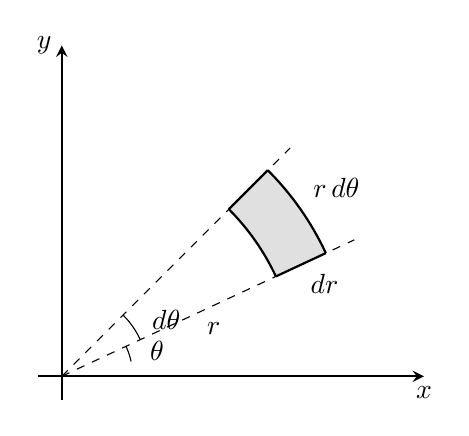
\begin{tikzpicture}[scale=1.0,>=stealth]
  \draw[thick,->] (-0.3,0) -- (4.6,0) node[below] {$x$};
  \draw[thick,->] (0,-0.3) -- (0,4.2) node[left] {$y$};
  \fill[black!12] (25:3) -- (25:3.7) arc[start angle=25,end angle=45,radius=3.7]
      -- (45:3) arc[start angle=45,end angle=25,radius=3];
  \draw[thick] (25:3) -- (25:3.7);
  \draw[thick] (45:3) -- (45:3.7);
  \draw[thick] (25:3) arc[start angle=25,end angle=45,radius=3];
  \draw[thick] (25:3.7) arc[start angle=25,end angle=45,radius=3.7];
  \draw[dashed] (0,0) -- (25:4.1);
  \draw[dashed] (0,0) -- (45:4.1);
  \draw[thin] (25:1.1) arc[start angle=25,end angle=45,radius=1.1];
  \node[right] at (35:1.25) {$d\theta$};
  \draw[thin] (12:0.9) arc[start angle=12,end angle=25,radius=0.9];
  \node[right] at (18:1.05) {$\theta$};
  \node[below right] at (25:3.35) {$dr$};
  \node[below right] at (25:1.9) {$r$};
  \node[above right] at (35:3.75) {$r\,d\theta$};
\end{tikzpicture}
\end{center}

$r$ থেকে $r+dr$ এবং $\theta$ থেকে $\theta+d\theta$-এর মধ্যেকার টুকরোটি দেখো।
তার একটি বাহু ব্যাসার্ধ বরাবর, দৈর্ঘ্য $dr$। অন্য বাহুটি চাপ বরাবর, আর
৭ নম্বর অধ্যায়ের radian-এর সংজ্ঞা অনুযায়ী তার দৈর্ঘ্য $r\,d\theta$।
টুকরোটি ঠিক আয়তক্ষেত্র নয়, ভেতরের চাপ বাইরেরটার চেয়ে সামান্য ছোট; কিন্তু
সেই পার্থক্যটুকু উচ্চতর ক্রমের (higher order term)  , তাই বাদ যায়।

\begin{idea}[ক্ষেত্রফল ও আয়তন উপাদান]
\[
  \mathrm{Cartesian:} \quad dA = dx\,dy, \qquad dV = dx\,dy\,dz ,
\]
\[
  \mathrm{Plane\ polar:} \quad dA = r\,dr\,d\theta ,
\]
\[
  \mathrm{Cylindrical\ } (s,\phi,z): \quad dV = s\,ds\,d\phi\,dz ,
\]
\[
  \mathrm{Spherical\ } (r,\theta,\phi): \quad
  dV = r^{2}\sin\theta\,dr\,d\theta\,d\phi .
\]
\end{idea}

Cylindrical-এরটা সহজ: $xy$-সমতলে টুকরোটির ক্ষেত্রফল $s\,ds\,d\phi$ (উপরের
polar হিসাবেই, কেবল নাম বদলে), আর উচ্চতা $dz$।

Spherical-এরটা একটু ভাবতে হয়, তাই ছবি দেখা যাক।

\begin{center}
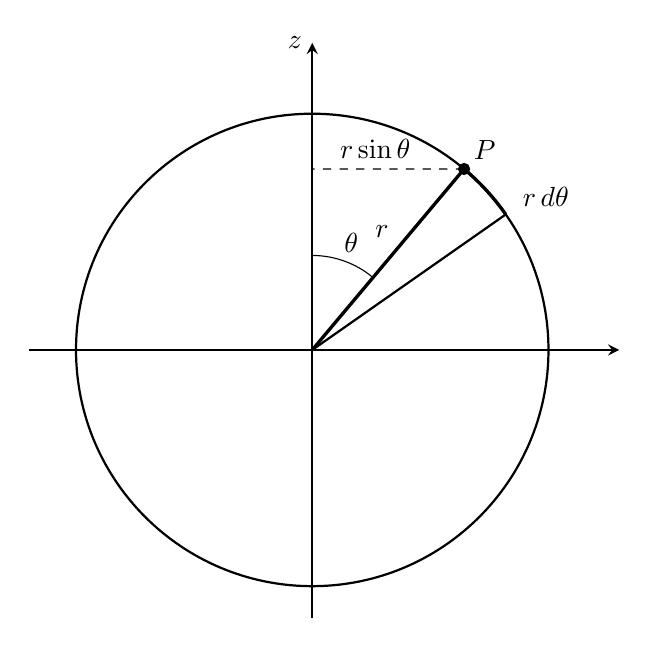
\begin{tikzpicture}[scale=1.0,>=stealth]
  \draw[thick,->] (0,-3.4) -- (0,3.9) node[left] {$z$};
  \draw[thick,->] (-3.6,0) -- (3.9,0);
  \draw[thick] (0,0) circle (3);
  \draw[very thick] (0,0) -- (50:3);
  \draw[thick] (0,0) -- (35:3);
  \draw[very thick] (50:3) arc[start angle=50,end angle=35,radius=3];
  \draw[fill] (50:3) circle (2pt) node[above right] {$P$};
  \draw[dashed] (50:3) -- (0,2.298);
  \draw[thin] (90:1.2) arc[start angle=90,end angle=50,radius=1.2];
  \node at (70:1.45) {$\theta$};
  \node[above left] at (50:1.7) {$r$};
  \node[right] at (2.55,1.95) {$r\,d\theta$};
  \node[above] at (0.8,2.31) {$r\sin\theta$};
\end{tikzpicture}
\end{center}

ছবিটি $z$-অক্ষ ধরে একটি মধ্যচ্ছেদ। টুকরোটির তিনটি বাহু:

এক, ব্যাসার্ধ বরাবর, দৈর্ঘ্য $dr$।

দুই, $\theta$ বাড়ানোর দিকে। এটি $r$ ব্যাসার্ধের একটি বৃত্তচাপ, তাই দৈর্ঘ্য
$r\,d\theta$ (ছবিতে মোটা চাপটি)।

তিন, $\phi$ বাড়ানোর দিকে, অর্থাৎ $z$-অক্ষকে ঘিরে ঘোরার দিকে। এখানেই সাবধান
হতে হয়: এই ঘূর্ণনের ব্যাসার্ধ $r$ নয়, বরং $z$-অক্ষ থেকে $P$-এর লম্ব দূরত্ব,
যা ছবির ভাঙা রেখাটি, অর্থাৎ $r\sin\theta$। সুতরাং বাহুটির দৈর্ঘ্য
$r\sin\theta\,d\phi$।

তিনটি বাহু পরস্পর লম্ব, তাই
\[
  dV = dr \cdot r\,d\theta \cdot r\sin\theta\,d\phi
     = r^{2}\sin\theta\,dr\,d\theta\,d\phi .
\]

দুটি যাচাই। এক, মাত্রা মেলে: তিনটি দৈর্ঘ্যের গুণফল। দুই, বিষুবরেখায়
($\theta = \pi/2$) $\sin\theta = 1$ এবং $r\sin\theta = r = s$, যা cylindrical
উপাদানের সঙ্গে মিলে যায়; আবার মেরুর কাছে ($\theta \to 0$) $\sin\theta \to 0$,
অর্থাৎ টুকরোগুলো সরু হয়ে আসে, যা ছবির সঙ্গেও মেলে।

\begin{remark}
১২ নম্বর অধ্যায়ের সতর্কবার্তাটি এখানে আবার কাজে লাগছে। গণিতের বইয়ে
spherical উপাদান লেখা থাকে $\rho^{2}\sin\phi\,d\rho\,d\phi\,d\theta$ আকারে,
কারণ সেখানে $\phi$ হলো $z$-অক্ষ থেকে মাপা কোণ। আমাদের নিয়মে ওই কোণটির নাম
$\theta$, তাই $\sin$-এর ভেতরে $\theta$ বসে। কোনো বই থেকে সূত্র তুলে আনার
আগে দেখে নাও তার ছবিতে কোন অক্ষর কোন কোণ; ভুল অক্ষরে $\sin$ বসালে গোটা হিসাব
ভুল হবে এবং ভুলটা ধরা কঠিন।
\end{remark}

\begin{example}
$R$ ব্যাসার্ধের একটি সমসত্ত্ব বৃত্তাকার চাকতির পৃষ্ঠ ঘনত্ব $\sigma$। একটি
ক্ষুদ্র টুকরোর ভর $dm$ লেখো, এবং $z$-অক্ষের (কেন্দ্র দিয়ে যাওয়া লম্ব অক্ষ)
সাপেক্ষে তার জড়তার ভ্রামকের অবদান $dI$ লেখো।
\end{example}

\begin{solbox}
Polar স্থানাঙ্ক নিই, কারণ চাকতিটির প্রতিসাম্য বৃত্তীয়। ক্ষুদ্র টুকরোর
ক্ষেত্রফল $dA = r\,dr\,d\theta$, তাই
\[
  dm = \sigma\,dA = \sigma\,r\,dr\,d\theta .
\]
জড়তার ভ্রামকের সংজ্ঞায় $r$ মানে ঘূর্ণন অক্ষ থেকে দূরত্ব; এখানে অক্ষটি
কেন্দ্র দিয়ে লম্ব, তাই ওই দূরত্ব ঠিক polar স্থানাঙ্কের $r$। সুতরাং
\[
  dI = r^{2}\,dm = \sigma\,r^{3}\,dr\,d\theta .
\]
এখানেই থামছি; এই রাশিটিকে $r = 0$ থেকে $R$ এবং $\theta = 0$ থেকে $2\pi$
পর্যন্ত যোগ করলে যে $\tfrac{1}{2}MR^{2}$ পাওয়া যায়, সেই যোগ করার কাজটি
১৭ নম্বর অধ্যায়ের।

লক্ষ করো, সেটআপের কঠিন অংশটা ছিল $dA$-তে $r$ গুণনীয়কটি মনে রাখা। ওটি ভুলে
$dA = dr\,d\theta$ লিখলে উত্তর ভুল আসত, এবং মাত্রা দেখেও ধরা যেত: $dr\,d\theta$
দৈর্ঘ্যের মাত্রা রাখে, ক্ষেত্রফলের নয়।
\end{solbox}

\prob{2} $x = 0$ থেকে $x = L$ পর্যন্ত বিস্তৃত একটি সরু দণ্ডের দৈর্ঘ্য ঘনত্ব
$\lambda(x) = \lambda_{0}\left( 1 + \dfrac{x}{L} \right)$।
\begin{enumerate}
  \item $x$ ও $x+dx$-এর মধ্যেকার টুকরোর ভর $dm$ লেখো।
  \item ওই টুকরোর ভরকেন্দ্র-ভ্রামকের অবদান, অর্থাৎ $x\,dm$, লেখো।
\end{enumerate}

\begin{sol}
\begin{enumerate}
  \item টুকরোটির দৈর্ঘ্য $dx$ এবং তার ভেতরে ঘনত্ব প্রায় ধ্রুবক, তাই
        \[
          dm = \lambda(x)\,dx
             = \lambda_{0}\left( 1 + \frac{x}{L} \right)dx .
        \]
  \item \[
          x\,dm = \lambda_{0}\left( x + \frac{x^{2}}{L} \right)dx .
        \]
\end{enumerate}
দুটিই কেবল সেটআপ; যোগ করার ধাপটি ১৭ নম্বর অধ্যায়ে।
\end{sol}

\prob{3} \begin{enumerate}
  \item ছবির যুক্তি ব্যবহার করে দেখাও যে plane polar স্থানাঙ্কে
        $dA = r\,dr\,d\theta$।
  \item $R$ ব্যাসার্ধের একটি চাকতির পৃষ্ঠ ঘনত্ব $\sigma(r) =
        \sigma_{0}\dfrac{r}{R}$। ক্ষুদ্র টুকরোর ভর $dm$ লেখো।
\end{enumerate}

\begin{sol}
\begin{enumerate}
  \item $r$ থেকে $r+dr$ এবং $\theta$ থেকে $\theta+d\theta$-এর মধ্যেকার
        টুকরোটির দুটি বাহু পরস্পর লম্ব: একটি ব্যাসার্ধ বরাবর, দৈর্ঘ্য $dr$;
        অন্যটি চাপ বরাবর, আর radian-এর সংজ্ঞা অনুযায়ী চাপের দৈর্ঘ্য
        $= $ ব্যাসার্ধ $\times$ কোণ $= r\,d\theta$। টুকরোটি ছোট হলে তাকে
        আয়তক্ষেত্র ধরা যায়, তাই ক্ষেত্রফল $r\,dr\,d\theta$।

        (ভেতরের চাপের দৈর্ঘ্য $r\,d\theta$ আর বাইরেরটির $(r+dr)\,d\theta$;
        পার্থক্যটি $dr\,d\theta$ ক্রমের, অর্থাৎ মূল রাশির তুলনায় ছোট, তাই
        বাদ যায়। এই ধাপটি এখানে ধরে নেওয়া হচ্ছে।)
  \item \[
          dm = \sigma(r)\,dA
             = \sigma_{0}\frac{r}{R} \cdot r\,dr\,d\theta
             = \frac{\sigma_{0}}{R}\,r^{2}\,dr\,d\theta .
        \]
\end{enumerate}
\end{sol}

\prob{3} $R$ ব্যাসার্ধের একটি গোলকের পৃষ্ঠে ক্ষুদ্র টুকরোর ক্ষেত্রফল
$dA = R^{2}\sin\theta\,d\theta\,d\phi$ হয়, দেখাও। এখান থেকে solid angle
উপাদান $d\Omega$ লেখো, এবং ১১ নম্বর অধ্যায়ের $\Omega = A/r^{2}$ সংজ্ঞার
সঙ্গে মিলিয়ে দেখাও যে পুরো গোলকের জন্য এটি $4\pi$ দেয়।

\begin{sol}
পৃষ্ঠের উপর $r = R$ ধ্রুবক, তাই $dr$ পদটি নেই এবং টুকরোটির কেবল দুটি বাহু:
$\theta$ দিকে $R\,d\theta$ এবং $\phi$ দিকে $R\sin\theta\,d\phi$। দুটি পরস্পর
লম্ব, সুতরাং
\[
  dA = R\,d\theta \cdot R\sin\theta\,d\phi = R^{2}\sin\theta\,d\theta\,d\phi .
\]

১১ নম্বর অধ্যায়ের সংজ্ঞা $\Omega = A/R^{2}$ ক্ষুদ্র টুকরোর জন্য লিখলে
\[
  d\Omega = \frac{dA}{R^{2}} = \sin\theta\,d\theta\,d\phi ,
\]
যেখানে $R$ কাটাকাটি গেছে, ঠিক যেমনটা হওয়ার কথা: solid angle দূরত্বের উপর
নির্ভর করে না।

পুরো গোলক পেতে $\theta$-কে $0$ থেকে $\pi$ এবং $\phi$-কে $0$ থেকে $2\pi$
পর্যন্ত নিতে হয়। যোগ করার কাজটি ১৭ নম্বর অধ্যায়ের, তবে ফলটি আগে থেকেই
জানা: গোলকের পৃষ্ঠতল $4\pi R^{2}$ (১১ নম্বর অধ্যায়), তাই
\[
  \Omega = \frac{4\pi R^{2}}{R^{2}} = 4\pi \ \mathrm{sr} ,
\]
যা মিলে যাচ্ছে।
\end{sol}

\prob{4} $R$ ব্যাসার্ধের একটি নিরেট গোলকের ঘনত্ব কেবল কেন্দ্র থেকে দূরত্বের
উপর নির্ভর করে: $\rho(r) = \rho_{0}\left( 1 - \dfrac{r}{R} \right)$।
\begin{enumerate}
  \item $r$ থেকে $r+dr$-এর মধ্যেকার পাতলা গোলীয় খোলের আয়তন $dV$ ও ভর $dm$
        লেখো। (ইঙ্গিত: গোটা খোলটিকে একসঙ্গে নাও, $\theta$ ও $\phi$ আলাদা করে
        রাখার দরকার নেই।)
  \item একটি পাতলা গোলীয় খোলের ভর $dm$ ও ব্যাসার্ধ $r$ হলে তার ব্যাস বরাবর
        অক্ষের সাপেক্ষে জড়তার ভ্রামক $dI = \tfrac{2}{3}r^{2}\,dm$ (এটি
        পদার্থবিজ্ঞান থেকে দেওয়া ধরে নাও)। গোটা গোলকের $I$ পাওয়ার জন্য যে
        রাশিটি যোগ করতে হবে সেটি লেখো।
\end{enumerate}

\begin{sol}
\begin{enumerate}
  \item খোলটির পৃষ্ঠতল $4\pi r^{2}$ এবং পুরুত্ব $dr$, তাই
        \[
          dV = 4\pi r^{2}\,dr .
        \]
        (একই ফল spherical উপাদান থেকেও আসে: $r^{2}\sin\theta\,dr\,d\theta\,
        d\phi$-কে $\theta$ ও $\phi$ জুড়ে যোগ করলে কোণীয় অংশটি $4\pi$ দেয়,
        আর $r^{2}\,dr$ থেকে যায়।) সুতরাং
        \[
          dm = \rho(r)\,dV
             = 4\pi\rho_{0}\left( 1 - \frac{r}{R} \right)r^{2}\,dr .
        \]
  \item \[
          dI = \frac{2}{3}r^{2}\,dm
             = \frac{8\pi\rho_{0}}{3}\left( 1 - \frac{r}{R} \right)r^{4}\,dr .
        \]
        এই রাশিটি $r = 0$ থেকে $R$ পর্যন্ত যোগ করলেই $I$ পাওয়া যাবে; সেই
        যোগটি ১৭ নম্বর অধ্যায়ের কাজ।
\end{enumerate}
খেয়াল করো, ঘনত্ব কেবল $r$-এর উপর নির্ভর করায় গোটা খোলটিকে একটিমাত্র টুকরো
ধরা গেল, আর তিন মাত্রার সমস্যাটি এক মাত্রায় নেমে এল। প্রতিসাম্য দেখে উপাদান
বেছে নেওয়া সেটআপের সবচেয়ে বড় কৌশল।
\end{sol}

\section{রৈখিক আসন্নীকরণ}

Differential-এর সবচেয়ে সরাসরি ব্যবহারটা এবার।

\begin{idea}[রৈখিক আসন্নীকরণ]
$f$ যদি $a$-তে differentiable হয়, তবে $a$-এর কাছে
\[
  f(x) \approx f(a) + f'(a)(x-a) ,
\]
অর্থাৎ $\Delta y \approx dy$। ডান পাশের রাশিটি হলো $x = a$ বিন্দুতে
স্পর্শকের সমীকরণ।
\end{idea}

এটি নতুন কিছু নয়; প্রথম অনুচ্ছেদের ছবিটিই এই কথা বলছিল, আর ১৫ নম্বর
অধ্যায়ের Taylor সিরিজের প্রথম দুটি পদও ঠিক এটাই। নতুন যা, তা হলো ব্যবহার।

\begin{example}
রৈখিক আসন্নীকরণ ব্যবহার করে $\sqrt{4.02}$-এর মান নির্ণয় করো।
\end{example}

\begin{solbox}
$f(x) = \sqrt{x}$ এবং $a = 4$ নিই, কারণ $\sqrt{4}$ আমরা জানি। তখন
$f'(x) = \dfrac{1}{2\sqrt{x}}$, তাই $f'(4) = \dfrac{1}{4}$। সুতরাং
\[
  \sqrt{4.02} \approx 2 + \frac{1}{4}(0.02) = 2 + 0.005 = 2.005 .
\]
প্রকৃত মান $2.0049938\ldots$, অর্থাৎ ভুল প্রায় $6 \times 10^{-6}$।

কৌশলটা মনে রাখো: এমন একটি $a$ বেছে নাও যেখানে উত্তর হাতে আছে এবং যা লক্ষ্যের
কাছে।
\end{solbox}

\begin{idea}[ত্রুটি নির্ণয়]
কোনো রাশি $x$ মাপা হয়েছে এবং তাতে সম্ভাব্য ত্রুটি $dx$। তাহলে $y = f(x)$-এ
সৃষ্ট ত্রুটি
\[
  dy \approx f'(x)\,dx .
\]
আপেক্ষিক ত্রুটি $\dfrac{dy}{y}$, আর একে $100$ দিয়ে গুণ করলে শতকরা ত্রুটি।
\end{idea}

দুটি বিশেষ ক্ষেত্র এত বেশি লাগে যে আলাদা করে মনে রাখা উচিত।

প্রথমত ঘাত। $y = x^{n}$ হলে $dy = nx^{n-1}dx$, তাই ভাগ করে
\[
  \frac{dy}{y} = n\,\frac{dx}{x} .
\]
অর্থাৎ আপেক্ষিক ত্রুটি ঘাত দিয়ে গুণ হয়ে যায়। ব্যাসার্ধে ১ শতাংশ ভুল থাকলে
আয়তনে ৩ শতাংশ।

দ্বিতীয়ত গুণফল। $y = uv$ হলে দুই পাশে $\ln$ নিয়ে (১০ নম্বর অধ্যায়)
$\ln y = \ln u + \ln v$, আর differential নিয়ে (১৫ নম্বর অধ্যায়ের
$\ln$-এর derivative)
\[
  \frac{dy}{y} = \frac{du}{u} + \frac{dv}{v} .
\]
অর্থাৎ গুণফলে আপেক্ষিক ত্রুটিগুলো যোগ হয়। ভাগফলেও তাই, কেবল চিহ্ন বদলে।

\begin{remark}
এখানে একটি সীমাবদ্ধতা স্পষ্ট করে বলা দরকার। উপরের নিয়মগুলো দেয় সবচেয়ে
খারাপ ক্ষেত্র, অর্থাৎ যদি সব ত্রুটি একসঙ্গে একই দিকে যায়। বাস্তবে মাপজোখের
ত্রুটিগুলো স্বাধীন ও এলোমেলো হয়, তাই তারা এভাবে সরল যোগ হয় না; তারা যোগ হয়
বর্গের যোগফলের মাধ্যমে। এখানে
যা শিখছ তা তার ভিত্তি: কোন রাশি কোন হারে ত্রুটি ছড়ায়, সেটা derivative-ই বলে
দেয়।
\end{remark}

\prob{2} রৈখিক আসন্নীকরণ ব্যবহার করে নির্ণয় করো: (ক) $\sqrt{101}$;
(খ) $\dfrac{1}{2.02}$।

\begin{sol}
(ক) $f(x) = \sqrt{x}$, $a = 100$, $f'(100) = \dfrac{1}{20}$। সুতরাং
\[
  \sqrt{101} \approx 10 + \frac{1}{20}(1) = 10.05 .
\]
প্রকৃত মান $10.0499$।

(খ) $f(x) = \dfrac{1}{x}$, $a = 2$, $f'(x) = -\dfrac{1}{x^{2}}$, তাই
$f'(2) = -\dfrac{1}{4}$। সুতরাং
\[
  \frac{1}{2.02} \approx 0.5 - \frac{1}{4}(0.02) = 0.495 .
\]
প্রকৃত মান $0.49505$।
\end{sol}

\prob{2} $30^{\circ}$-এর চারপাশে রৈখিক আসন্নীকরণ ব্যবহার করে
$\sin 31^{\circ}$ নির্ণয় করো। ($\sin 30^{\circ} = 0.5$,
$\cos 30^{\circ} = 0.86603$।)

\begin{sol}
প্রথমে radian-এ কাজ করতে হবে, কারণ derivative-এর সূত্র radian ধরে
(১৫ নম্বর অধ্যায়)। $a = \dfrac{\pi}{6}$ এবং
\[
  dx = 1^{\circ} = \frac{\pi}{180} = 0.0174533 .
\]
সুতরাং
\[
  \sin 31^{\circ} \approx \sin 30^{\circ} + \cos 30^{\circ} \cdot dx
  = 0.5 + 0.86603 \times 0.0174533 = 0.515115 .
\]
প্রকৃত মান $0.515038$, অর্থাৎ ভুল প্রায় $0.015$ শতাংশ।

ডিগ্রিতে $dx = 1$ বসালে উত্তর আসত $1.366$, যা অর্থহীন; radian-এ বদলানোর
ধাপটিই এখানে আসল।
\end{sol}

\prob{3} একটি গোলকের ব্যাসার্ধ মাপা হলো $10.0$ সেমি, সম্ভাব্য ত্রুটি
$0.1$ সেমি।
\begin{enumerate}
  \item আয়তনের সর্বোচ্চ ত্রুটি ও শতকরা ত্রুটি নির্ণয় করো।
  \item পৃষ্ঠতলের ক্ষেত্রে একই দুটি নির্ণয় করো।
\end{enumerate}

\begin{sol}
\begin{enumerate}
  \item $V = \tfrac{4}{3}\pi r^{3}$, তাই $\dfrac{dV}{V} = 3\dfrac{dr}{r}
        = 3 \times \dfrac{0.1}{10} = 0.03$, অর্থাৎ ৩ শতাংশ।

        মান: $V = \tfrac{4}{3}\pi(1000) = 4188.8$ ঘন সেমি, তাই
        $dV = 0.03 \times 4188.8 \approx 126$ ঘন সেমি।
  \item $A = 4\pi r^{2}$, তাই $\dfrac{dA}{A} = 2\dfrac{dr}{r} = 0.02$,
        অর্থাৎ ২ শতাংশ। $A = 4\pi(100) = 1256.6$ বর্গ সেমি, তাই
        $dA \approx 25$ বর্গ সেমি।
\end{enumerate}
এক শতাংশ ভুল মাপা ব্যাসার্ধ আয়তনে তিন গুণ বড় ভুল তৈরি করছে; ঘন রাশি মাপার
সময় তাই দৈর্ঘ্য মাপায় বাড়তি যত্ন লাগে।
\end{sol}

\prob{4} $k$ ধ্রুবক এবং $y = k\,u^{a}v^{b}w^{c}$।
\begin{enumerate}
  \item দেখাও যে
        $\dfrac{dy}{y} = a\dfrac{du}{u} + b\dfrac{dv}{v} + c\dfrac{dw}{w}$।
  \item সরল দোলকের পর্যায়কাল $T = 2\pi\sqrt{\dfrac{L}{g}}$। $L$ মাপায়
        ১ শতাংশ এবং $g$-তে ২ শতাংশ ত্রুটি থাকলে $T$-তে সর্বোচ্চ শতকরা
        ত্রুটি কত?
\end{enumerate}

\begin{sol}
\begin{enumerate}
  \item দুই পাশে $\ln$ নিই:
        \[
          \ln y = \ln k + a\ln u + b\ln v + c\ln w .
        \]
        এবার differential নিই; $\ln$-এর derivative $1/x$ (১৫ নম্বর
        অধ্যায়), আর $\ln k$ ধ্রুবক বলে তার differential শূন্য:
        \[
          \frac{dy}{y} = a\frac{du}{u} + b\frac{dv}{v} + c\frac{dw}{w} .
        \]
  \item $T = 2\pi L^{1/2}g^{-1/2}$, তাই উপরের সূত্রে $a = \tfrac{1}{2}$ ও
        $b = -\tfrac{1}{2}$:
        \[
          \frac{dT}{T} = \frac{1}{2}\frac{dL}{L} - \frac{1}{2}\frac{dg}{g} .
        \]
        সর্বোচ্চ ত্রুটির জন্য দুটি অবদানের \emph{মান} যোগ করি (কারণ চিহ্ন
        কোন দিকে যাবে তা জানা নেই):
        \[
          \left| \frac{dT}{T} \right|_{\max}
          = \frac{1}{2}(0.01) + \frac{1}{2}(0.02) = 0.015 ,
        \]
        অর্থাৎ ১.৫ শতাংশ।
\end{enumerate}
এটি সবচেয়ে খারাপ ক্ষেত্রের হিসাব। 
\end{sol}

\end{document}